\begin{frame}{browsers and website leakage}
    \begin{itemize}
    \item web browsers run code from untrusted webpages
    \item one goal: can't tell what other webpages you visit
    \end{itemize}
\end{frame}

\begin{frame}[fragile]{some webpage leakage (1)}
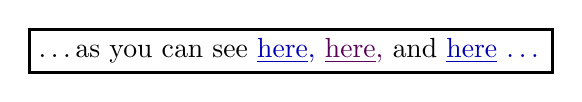
\begin{tikzpicture}
\node[draw,very thick] {
    \ldots as you can see \color{blue!70!black}{\underline{here}}, \color{violet!70!black}{\underline{here}},
    \color{black!70!black}{and} \color{blue!70!black}{\underline{here}} \ldots
};
\end{tikzpicture}
\begin{itemize}
\item convenient feature 1: browser marks visited links
\end{itemize}
\begin{tikzpicture}
\node[draw,very thick,align=left] {
\begin{lstlisting}[style=smaller,language={}]
<script>
var the_color = window.getComputedStyle(
    document.querySelector('a[href=~"foo.com"]')
).color
if (the_color == ...) { ... }
</script>
\end{lstlisting}
};
\end{tikzpicture}
\begin{itemize}
\item \sout<2->{convenient feature 2: scripts can query current color of something}
    \begin{itemize}
    \item<2-> fix 1: getComputedStyle lies about the color
    \item<2-> fix 2: limited styling options for visited links
    \end{itemize}
\end{itemize}
\end{frame}

\begin{frame}{some webpage leakage (2)}
\begin{itemize}
\item one idea: script in webpage times loop that writes big array
\item variation in timing depends on \myemph{other things running on machine}
\end{itemize}
\begin{tikzpicture}
\begin{visibleenv}<2->
\node (pic) {
\includegraphics[height=0.6\textheight]{../spectre/website-sigs-fig}
};
\node[anchor=north west,align=left] at (pic.north east) {
turns out, other webpages \\
create distinct ``signatures'' \\
\fontsize{8}{9}\selectfont\parbox{10cm}{Figure from Cook et al, ``There’s Always a Bigger Fish:
Clarifying Analysis of a Machine-Learning-Assisted Side-Channel Attack'' (ISCA '22)}
};
\end{visibleenv}
\end{tikzpicture}
\end{frame}
